
\subsection{System Risk}
\begin{frame}{Current Models}
Determinsitic has fixed line thresholds
\bi
\item Line is completely okay
\item or system is infeasible
\ei
\pause
Chance Constraints
\bi
\item Enforce line threshold probalistically
\ei
\pause

\alert{Line thresholds are soft constraints in real life}
\pause
\bi
\item Multiple line ratings (i.e. short term emergency rating)
\item Hard limit typically relay tripping
\ei
\end{frame}

\begin{frame}{Line Limits}
Limited by
\bi
\item Sagging due to current flow and line heating
\item \alert<2>{Worst case environmental conditions (seasonally)}
\item An acceptable probability of line failure
\item Enforce N-1 Reliability Constraint
\ei
\bigskip
\pause
\textbf{Dynamic line limits}
\bi
\item Real time limits based on current environmental conditions
\ei

\end{frame}

\begin{frame}{System Risk}

System risk related to line loadings (severity measure) \footnotemark
%\footfullcite{wang_2013}
\footnotetext[2]{Qin Wang and McCalley, J.D. and Tongxin Zheng and Litvinov, E.}
\pause


\BBR{\textbf{System Risk} Probability of line failure}
\begin{equation*}
 h(y) = P_\Xi \left[ \mbox{at least one line fails} | y \right] 
\end{equation*}
\EBR
\pause

\vspace{10pt}
Intuition
\bi
\item Grid relatively stressed when more lines are near their limit
\ei
%Want risk measure to compare risk of line loadings
%\vspace{10pt}
\end{frame}

\begin{frame}{Line Risk Function}
Risk function takes the normalized flow returns line risk 
\begin{equation*}
 g(\hy_e) = \bP{\Xi}{\text{Line }e\text{ fails} | \hy_e} 
\end{equation*}
\pause
Piece-wise linear function choosen
\bi
\item Below $L$, there is no risk associated with loading
\item After $L$, the risk increases linearly with loading
\item At critical capacity $U^c$, line fails with certainty
\ei
\pause
\begin{equation*}
g(\hy_e) = \left\{ \begin{array}{l l}
  0 & \hy_e \leq L \\
  a + b \hy_e & L \leq \hy_e < U^c \\
  1 & U^c \leq \hy_e 
\end{array}
\right.
\end{equation*}
\end{frame}


\begin{frame}{System Risk, Fixed Injects}
\textbf{System Risk} Probability that at least one line fails
\begin{equation*}
 h(y) = P_\Xi \left[ \mbox{at least 1 line fails} \right] 
\end{equation*}
\pause
With fixed line flows, independent failures
\begin{equation*}  
h(y) = 1 - \prod_{e \in \cE} \left( 1 - g(y_e) \right)
\end{equation*}  
\pause
\bi
\item Implies hard line constraint, line risk=system risk
\item $h(y) \leq \epsilon$ not convex
\bi
\item But it is log convex, log transform and solve
\ei
\ei

\end{frame}

\begin{frame}{Gaussian Flow and Risk Function}
\begin{center}
\begin{tabular}{c c}
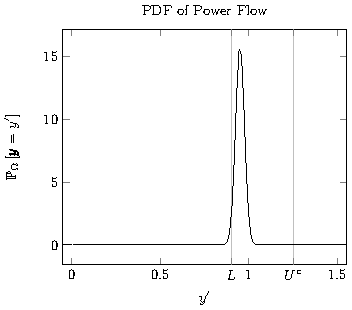
\includegraphics[scale=.8]{fig-pdfflow}
&
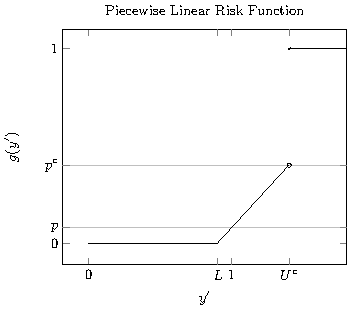
\includegraphics[scale=.8]{fig-failuredensity}\\
\hspace{10pt}Gaussian branch flow & \hspace{10pt}Line risk function 
\end{tabular}
\end{center}
\end{frame}


\begin{frame}{System Risk Under Uncertainty}
\vspace{10pt}
\BBR{Line Risk Function}
\begin{equation*}
\rho(\mu^y_e,\sigma^y_e) \equiv \E{\Omega}{g(\ry_e)}
\end{equation*}
\EBR
Function representation
\[ \rho(\mu^y_e,\sigma^y_e) = (a + b \mu^y_e)\left[ 1 - \Phi(\alpha_L) \right]  + b \sigma^y_e \phi(\alpha_L) \]

Function is
\pause
\bi
\item Convex with respect to $\mu^y_e, \sigma^y_e$ of branch flow $\ry_e$
\bi
\item $\sigma$ second order cone representable
\ei
\item Not expressable due to CDF of standard normal evaluation
\bi
\item Derivatives expressable
\ei
\ei
\pause
Solve with \alert{Cutting Planes!}



\end{frame}